\documentclass[12pt]{article}
\usepackage[czech]{babel}
\usepackage[T1]{fontenc}
\usepackage[utf8]{inputenc}
\usepackage{expl3}
\usepackage[a4paper, left=2cm, text={17cm, 25cm}, top=2.5cm]{geometry}
\usepackage[backend=biber,style=alphabetic,sorting=ynt]{biblatex}
\usepackage{listings}
\usepackage[czech]{babel}

\selectlanguage{czech}

\addto\captionsczech{\renewcommand{\figurename}{Obrázek}}

\addbibresource{bib.bib}

%\newcommand{\todo}[1]{\textcolor{red}{\textbf{[[#1]]}}}

\usepackage{relsize}

\usepackage{enumitem}
\setlist[description]{style=nextline}

\usepackage{url}

\usepackage{graphicx}

\usepackage[unicode, colorlinks]{hyperref}
\usepackage[all]{hypcap}

\begin{document}

\begin{titlepage}
    \begin{center}
        \Huge
        \textsc{Vysoké učení technické v~Brně} \\
        \huge
        \textsc{Fakulta informačních technologií} \\
        \vspace{\stretch{0.252}}
       
        	
\includegraphics[width=0.7\textwidth]{img/logo.png}
        
        \vspace{\stretch{0.382}}
        \Huge 
        Blockchainy a decentralizované aplikace \\
        \huge \smaller
        \vspace{\stretch{0.1}}
        Platforma na monitorování uzlů v P2P síti DASH \\
        \vspace{\stretch{0.618}}
    \end{center}
    \Large
    \null \hfill Bc. Daniel Pátek (\texttt{xpatek08}) \\
\end{titlepage}

\section{Kryptoměna DASH a její síť}
Kryptoměna DASH je ve své podstatě kopie kryptoměny Bitcoin. Vznikla v roce 2014 a došlo k tomu právě kopií existujícího Bitcoinu. Do dnešního dne se drží Bitcoinu velmi blízko jak ve fungování protokolu P2P sítě, tak v implementaci například RCP (Remote Procedure Calls). \cite{DashWiki}

\subsection{Připojování k síti}
Pokud se někdo rozhodne si spustit svůj vlastní uzel v síti DASH, se samotnou instalací by neměl mít žádný problém. Pro provoz klienta je potřeba stáhnout balíček s programem \textit{Dashcore}, respektive \textit{dashd}. \cite{Dashcore} Následně se vytvoří konfigurační soubor \texttt{dash.conf}, který obsahuje základní informace, jakým způsobem bude spuštěný klient pracovat. \cite{DashConf} Tento soubor je potřeba uložit mezi konfigurační soubory v operačním systému, typicky \texttt{\$HOME/.dashcore/dash.conf}.

\begin{lstlisting}[language=Python, caption=\texttt{dash.conf} použito v v projektu]
prune=1000
rpcuser=user
rpcpassword=passw
listen=1
server=1
rest=1
\end{lstlisting}

\noindent Důležitou volbou je takzvaný \textit{prune mode}, který umožní spustit uzel bez nutnosti synchronizace celého blockchainu na lokální disk. Nutno dodat, že takový klient nemůže potvrzovat transakce. Také je potřeba nastavit hodnotu proměnné \textit{server} na 1 pro spuštění RCP serveru.
Po takovém nastavení se uzel může spustit příkazem \texttt{./dashd} a uzel se sám připojí na několik dalších uzlů, které vyhledá automaticky pomocí DNS záznamů. \cite{DashDisc}

\subsection{RPC metody}
Nedílnou součástí komunikace mezi programem a uzlem je využití \textit{Remote procedure calls}. \cite{DashRPC} Tyto metody umožňují efektivní a rychlou komunikaci a využívají \textit{JSON-RPC}. \cite{jsonrpc} Jsou zde zmíněny a objasněny alespoň metody použité v projektu.

\begin{itemize}
    \item \textbf{\texttt{getpeerinfo}} - Vrátí informace o každém aktuálně připojeném peeru (uzlu).
    \item \textbf{\texttt{addnode}} - Využivá se buď pro přidání uzlu mezi uložené, nebo pro pokus o připojení se k tomuto uzlu.
    \item \textbf{\texttt{getnodeaddresses}} - Vrátí požadovaný počet nových adres uzlů získaných od připojených peerů.
\end{itemize}

\noindent Zde je nutné zmínit, že metoda \texttt{getnodeaddresses} v době tvorby tohoto projektu není dostupná v aktuální verzi \textit{Dashcore} 17. Z tohoto důvodu pro účely tohoto projektu budu využívat beta verzi \textit{Dashcore} 18, kde je již tato metoda funkční. Verze 18 je momentálně ve fázi finálního testování a její plné nasazení je očekáváno koncem května roku 2022. \cite{Dash18}

\newpage

\section{Návrh programu pro monitorování dostupných uzlů}

Hlavní program (v diagramu \ref{fig:navrh} níže označen jako \textit{Node Explorer App}) je navržen jako soubor čtyř na sobě nezávislých služeb. Pro persistenci dat byla zvolena databáze \textit{MongoDB}, hlavně kvůli své dobré škálovatelnosti při práci s mnoha záznamy. Součástí návrhu je i webová aplikace, která bude zobrazovat současný stav systému a umožní procházet získaná data o dalších uzlech.

\begin{figure}[ht]
	\centering
	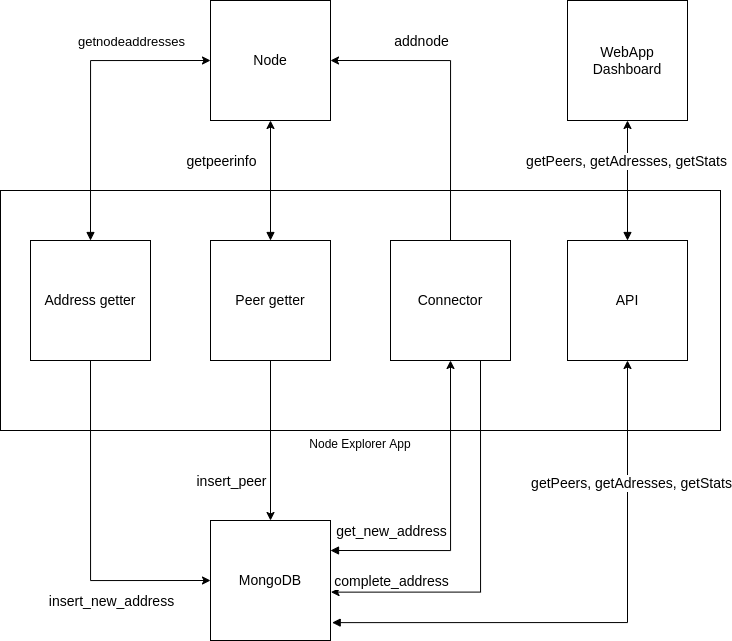
\includegraphics[width=0.90\textwidth]{img/components.png}
	\caption{Návrh jednotlivých komponent programu}
	\label{fig:navrh}
\end{figure}

\subsection{Představení jednotlivých částí programu}

\begin{itemize}
    \item \textbf{Node} - Jedná se o klienta \textit{Dashcore} s běžícím RPC serverem pro komunikaci s ostatními částmi programu.
    \item \textbf{MongoDB} - Databáze, která uchovává informace o adresách a uzlech v síti.
    \item \textbf{Address getter} - Tato služba komunikuje s částí \textbf{Node} a stará se o získávání dostupných adres pomocí RPC metody \texttt{getnodeaddresses} a následně jejich nahrání do databáze \textit{MongoDB}.
    \item \textbf{Peer getter} - Hlavním úkolem této služby je také komunikace s částí \textbf{Node}. Používá RPC metodu \texttt{getpeerinfo} pro získání informací o připojených uzlech a tyto informace následně nahrává do databáze.
    \item \textbf{Connector} - Navazování nových spojení řeší tato část programu. Nejprve si z databáze \textbf{MongoDB} vezme jednu adresu potencionálního uzlu v síti. RPC metodou \texttt{addnode} s argumentem \texttt{onetry} požádá část \textbf{Node} o připojení nového uzlu. Zároveň tuto adresu v databázi označí jako hotovou.
    \item \textbf{API} - Jedná se o funkční server s endpointy pro získávání informací, jako je seznam uzlů nebo seznam adres, z databáze \textbf{MongoDB}. Tuto službu využívá jen webová aplikace.
    \item \textbf{WebApp Dashboard} - Webová aplikace, která zobrazuje dostupné informace o programu, ale také aktuální stav uzlů v databázi.
\end{itemize}

\section{Výsledky}
Na základě požadavků byl implementován program pro monitorování dostupných uzlů v P2P síti kryptoměny DASH. Byl zvolen jazyk \textit{Python 3.8}. Webová aplikace byla implementována ve frameworku \textit{Next.js} jazyka \textit{JavaScript}.

\begin{figure}[ht]
	\centering
	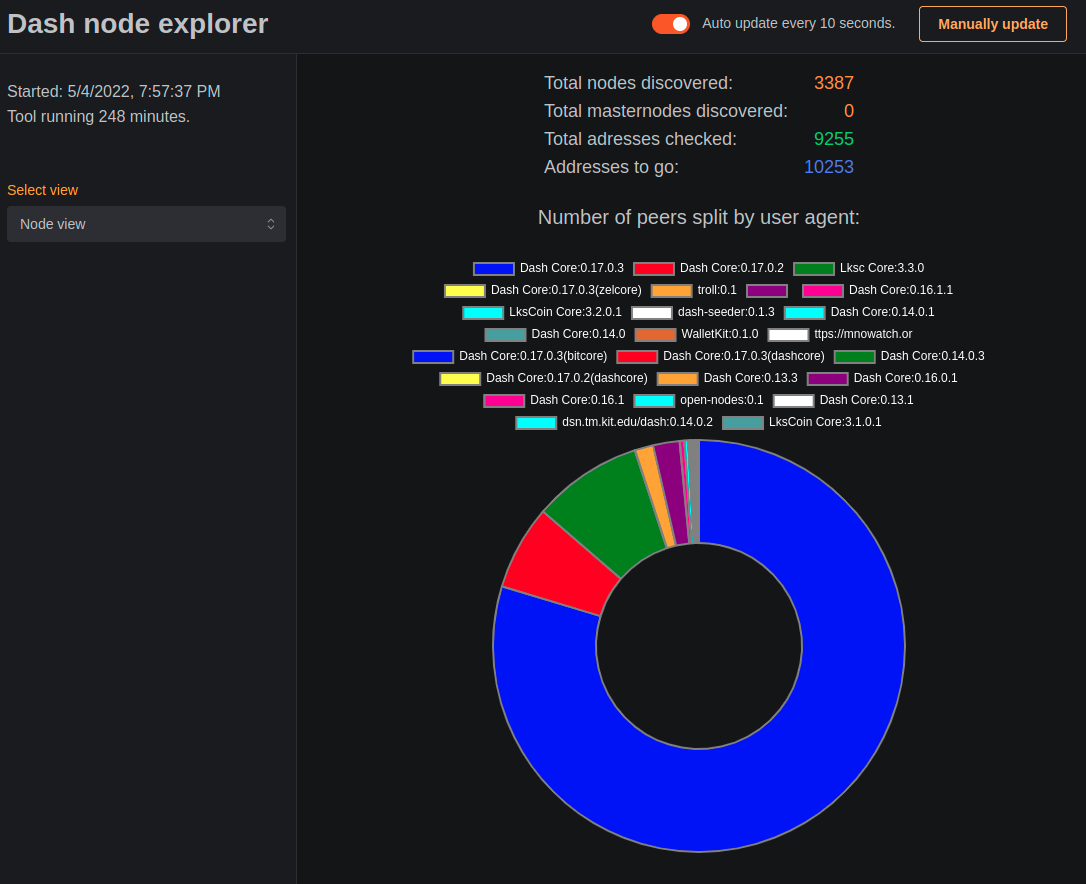
\includegraphics[width=0.90\textwidth]{img/web_app.png}
	\caption{Snímek obrazovky výsledné webové aplikace - dashboard}
	\label{fig:web_app_1}
\end{figure}

\noindent Jak by se dalo odvodit z Obrázku \ref{fig:web_app_1}, program byl ponechán zapnutý po dobu 4 hodin a 15 minut. Za tuto dobu bylo zpracováno 9255 různých adres uzlů v síti. Bylo navázáno 3387 spojení s dostupnými uzly a informace o těchto uzlech uloženy do databáze. V databázi se v tu dobu nacházelo ještě 10253 adres, které zatím nebyly vyzkoušeny na připojení.

\newpage

\begin{figure}[ht]
	\centering
	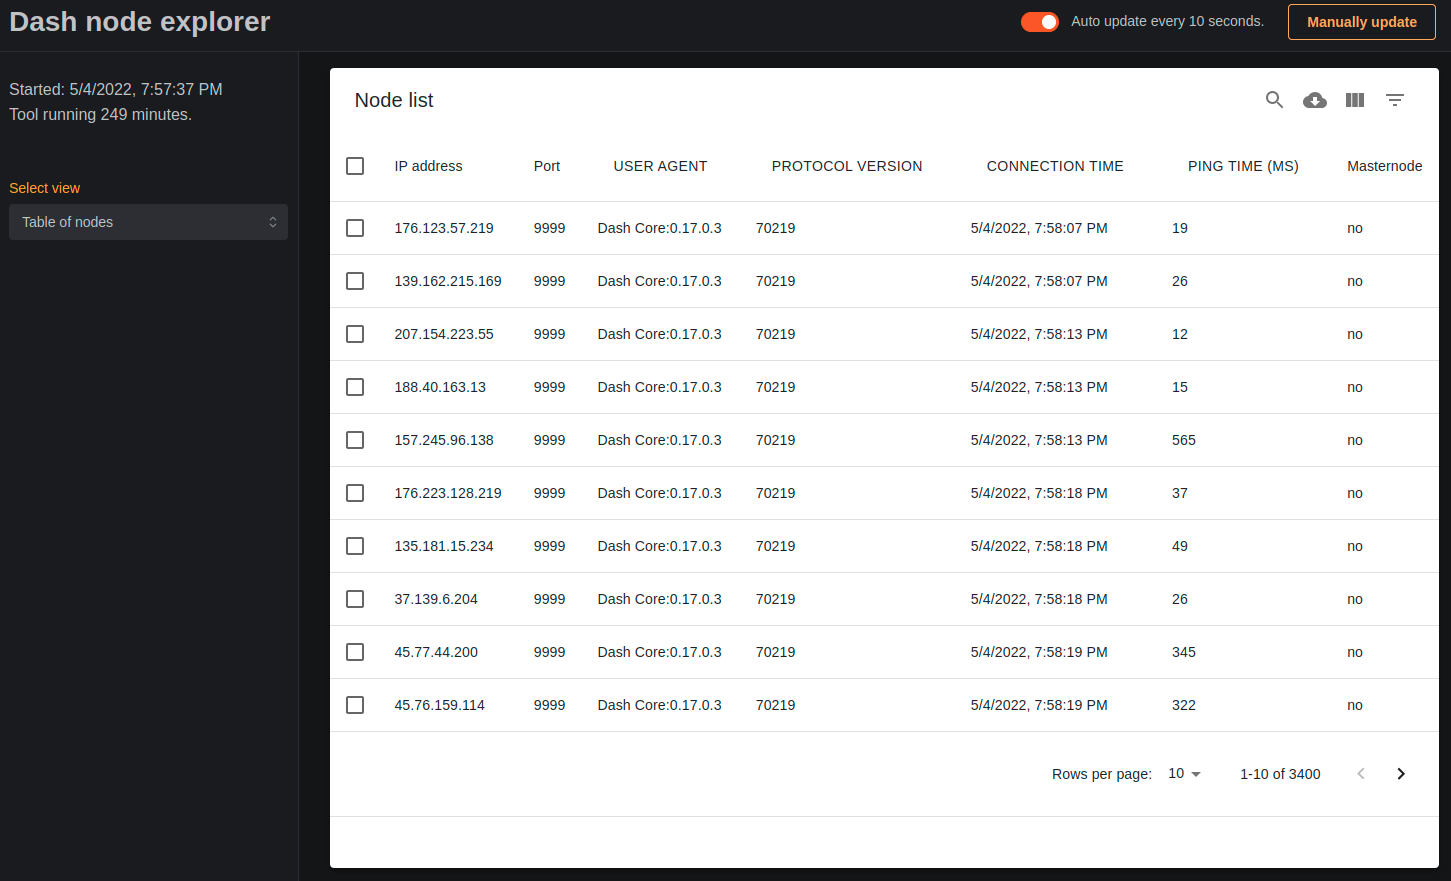
\includegraphics[width=0.95\textwidth]{img/web_app_2.png}
	\caption{Snímek obrazovky výsledné webové aplikace - tabulka}
	\label{fig:web_app_2}
\end{figure}

\noindent Pro zobrazení tabulky na obrázku \ref{fig:web_app_2} byla využita knihovna \textit{mui-datatables}. Tato knihovna obsahuje filtrování, řazení a také export dat do formátu \texttt{.csv} pro pohodlnou práci s informacemi.

\section{Zhodnocení}
Tento projekt byl bezesporu velmi zajímavý, ať už co se týče práce s kryptoměnovým klientem nebo získávání informací o připojených uzlech v síti.

\noindent Podařilo se mi sestavit funkční systém, který postupně mapuje uzly v P2P síti kryptoměny DASH a ukládá je do databáze. Implementoval jsem i webovou aplikaci pro přehledný přístup k těmto informacím.

\noindent Pokud bych měl tento projekt tvořit podruhé nebo například pro jinou kryptoměnu, určitě bych daleko více času věnoval studování dokumentace daného klienta kryptoměny. Nejednou se mi stalo, že jsem se v implementaci zasekl u nějakého bodu, který byl dobře objasněn právě v dokumentaci, i když třeba pod jinou záložkou, než jsem si v tu chvíli myslel.

\noindent Další bod, který bych změnil v mém implementačním postupu je \textit{dockerizace} programu včetně klienta \textit{Dashcore}. Věnoval jsem velké úsilí tomuto procesu hned na začátku, kdy jsem ještě zdaleka neměl hotový ani samotný program, bohužel bezúspěšně. U takového programu složeného z více nezávislých služeb je \textit{dockerizace} jistě žádoucí.

\newpage
\printbibliography

\end{document}